\chapter{BigTent解説}
OpenStackはそれぞれのコンポーネントが疎結合であるため、連携が容易であることが利点の1つです。その結果、さまざまな連携プロジェクトが生まれ、非常にリッチなクラウド環境の構築ができるようになりました。品質を維持するために、APIの仕様はきちんと議論された上で定義されます。それぞれのコンポーネントでバージョンを一致させ、結合テストを行います。が、つまりは増えすぎました。さまざまな派生プロジェクト間での調整を行うことが難しくなり、足並みをそろえるだけで数ヶ月かかるようになっていまいました。そこで、OpenStackのコアとなるコンポーネントを定義し、それらの結合テスト以外はサブプロジェクトとして、リリースを一致させる必要はない、ということにしました。これをOpenStack界隈では「BigTent構想」と言っています。

とはいえ、プロジェクトを減らそうという話ではないわけなので、相変わらずたくさんのプロジェクトが乱立しています。そんなわけで、サブプロジェクトの一部を紹介してみることにしました。プロジェクトのリストはOpenStackのWikiでまとめられているのですが、すべて英語なので調べる気が起きていないひともいるかと思います。

中には単一ベンダーが1人で頑張っているだけのプロジェクトもあります。また、機能が重複しているんじゃないかというプロジェクトもあります。ちゃんとWikiが整備されていなかったり説明が無かったりと、BigTentは玉石混交です。

\section{CloudKitty}
\begin{description}
	\item[wiki:] \url{https://wiki.openstack.org/wiki/CloudKitty}
	\item[開発者向けドキュメント:] \url{http://docs.openstack.org/developer/cloudkitty/}
	\item[IRC:] \verb|#cloudkitty| on freenode
\end{description}
Rating-as-a-serviceと説明されていますが、課金管理をしてくれます。さまざまなメトリクスを収集し、課金ルールを定義することができます。とあるITコンサルで開発されていたものをアトランタサミットでプロトタイプを紹介してみたところ、思ったより反応が良かったのでOpenStackのプロジェクトとしてオープンに開発していくことにしたようです。

一般的に課金ルールや配賦方法は、技術的というよりはビジネス的な要件から発生し、その手法もさまざまです。そのため、一般的な課金・配賦ルールはビルトインで定義されているものの、プラグイン型式で独自のルールを組み込むこともできるようになっています。Horizonとの統合も当初から設計されています。

Ceilometerは確かにメトリクスを計測してくれるのですが、課金に関してはそのスコープ外でした。CloudKittyは以下のプロセスから構成されています。

\begin{itemize}
	\item 課金のもととなるデータ (collector)
	\item 課金ポリシー (rating pipeline)
	\item 課金情報の保管 (storage)
	\item 書き出し (writers)
\end{itemize}

複数のコレクターや書き出しフォーマットを選ぶことができます。

\section{Congress}
\begin{description}
	\item[wiki:] \url{https://wiki.openstack.org/wiki/Congress}
	\item[IRC:] \verb|#congress| on freenode
\end{description}
OpenStackで構成されたインフラにガバナンスを効かせるためのコンポーネントです。と、wikiには書いてありますが、イメージが掴みにくいですね。文章量もかなりあるのですが。

物理プロビジョンニングが主流だった時代と異なり、仮想的なリソースを管理するためには運用ルールを徹底させるには、その自動化が必要になります。仮想マシンを1つ作るだけで毎回コアファイヤーウォール設定変更の許可を書類でもらうようなことは考えたくありません。Congressはネットワークやコンピュートリソース、ネットワークリソースに対してのガバナンスフレームワークをオープンソースコミュニティで開発していこうとするプロジェクトです。例えば

\begin{itemize}
	\item アプリケーションAはアプリケーションBとの通信のみ許可される
	\item テナントAがBグループの場合のみ、テナントAの仮想マシンはパブリックネットワークに接続される
	\item 仮想マシンAは物理的距離の遠いストレージBはマウントできない
\end{itemize}

などのルールを設定することができます。これらのルールをDatalog型式で記述します。

\section{Designate}
\begin{description}
	\item[wiki:] \url{https://wiki.openstack.org/wiki/Designate}
	\item[IRC:] \verb|#openstack-dns| on freenode
\end{description}

\begin{wrapfigure}[3]{r}[0mm]{0.3\textwidth}
	\begin{center}
		
\includegraphics[width=0.3\textwidth]{img/logo-designate.pdf}
	\end{center}
\end{wrapfigure}

みんな大好きDNSのサービスです。

\begin{itemize}
	\item ドメインとレコードの管理ができるAPIの提供
	\item マルチテナントのサポート
	\item Keystoneでの認証
	\item NovaやNeutronと連携してレコードの自動追加
\end{itemize}

いまのところPowerDNSとBIND9をインストール時点でサポート。プラグイン型式で追加も可能のようです。アーキテクチャはwikiで説明されています。

\begin{figure}
	\begin{center}
		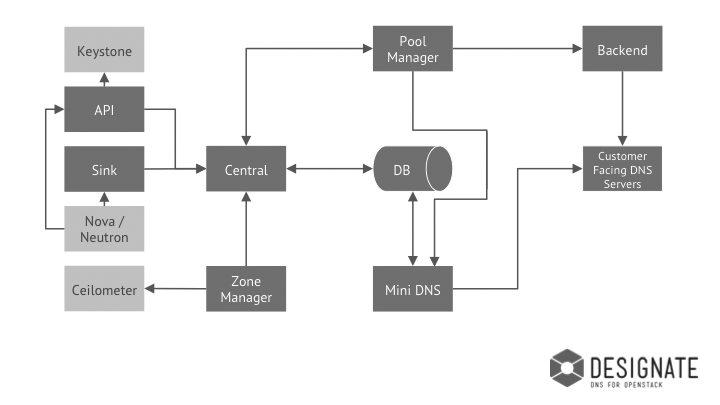
\includegraphics[width=\textwidth]{img/Designate-Arch.png}
	\end{center}
\end{figure}

\begin{description}
	\item[API:] APIリクエストを受け付けるプロセスです。認証はKeystoneへ、実際の操作はMQへ転送します。
	\item[Central:] MQからイベントを受け取ります。DNS操作を行うというよりは、Designateデータベースへの書き込みを担当します。レコード操作は別のプロセスが行います。
	\item[MiniDNS:] \verb|DNS NOTIFY|の送信や\verb|AXFR|に答えたりします。
	\item[Pool Manager:] Designate管理下にあるDNSを記憶し、同期することが責務です。
	\item[Zone Manager:] DNSの状態やゾーンの状態を定期的に監視し、Ceilometerなどに保存します。
	\item[Sink:] NovaやNeutronからのイベントを待ちます。
	\item[DNS Backend:] PowerDNS、BINDなど、実際にネームサービスを提供するサーバーです。
\end{description}

実際のコマンド例を見てみるとイメージしやすいでしょうか。ドメインの作成とレコードの作成は以下のようになるようです。

\begin{lstlisting}
$ designate domain-create --name designate-example.com. --email designate@example.org
+-------------+--------------------------------------+
| Field       | Value                                |
+-------------+--------------------------------------+
| description | None                                 |
| created_at  | 2015-02-13T16:23:26.533547           |
| updated_at  | None                                 |
| email       | designate@example.org                |
| ttl         | 3600                                 |
| serial      | 1423844606                           |
| id          | ae59d62b-d655-49a0-ab4b-ea536d845a32 |
| name        | designate-example.com.               |
+-------------+--------------------------------------+

$ designate record-create ae59d62b-d655-49a0-ab4b-ea536d845a32 --name www.designate-example.com. --type A --data 192.0.2.1
+-------------+--------------------------------------+
| Field       | Value                                |
+-------------+--------------------------------------+
| description | None                                 |
| type        | A                                    |
| created_at  | 2015-02-13T16:43:10.952601           |
| updated_at  | None                                 |
| domain_id   | ae59d62b-d655-49a0-ab4b-ea536d845a32 |
| priority    | None                                 |
| ttl         | None                                 |
| data        | 192.0.2.1                            |
| id          | 10b31f72-2358-466c-90d2-79aa015fbea4 |
| name        | www.designate-example.com.           |
+-------------+--------------------------------------+
\end{lstlisting}

プライベートDNSはなかなか自動化が進まなかったりする分野ではあるのですが、ニーズもまた大きいと思います。クラウドネイティブ、という考えからするとDNSに依存するのはあまり得策ではないのですが……。とはいえやはりDNSは必要な環境も多いだろうと思うので、注目されているコンポーネントでしょう。

\section{Dragonflow}

\begin{description}
	\item[wiki:] \url{https://wiki.openstack.org/wiki/Dragonflow}
	\item[wiki:] \url{http://docs.openstack.org/developer/dragonflow/}
	\item[IRC:] \verb|#openstack-dragonflow|
\end{description}

\begin{wrapfigure}[4]{r}[0mm]{0.3\textwidth}
	\begin{center}
		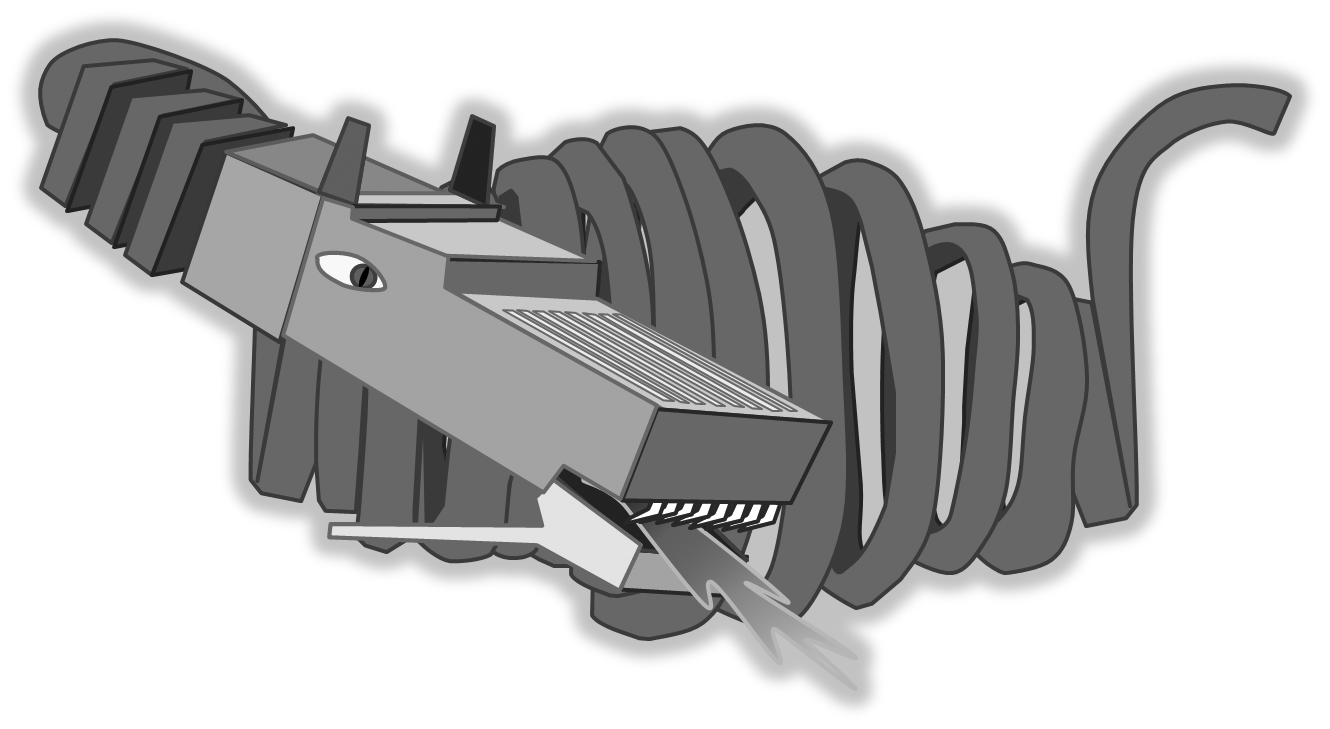
\includegraphics[width=0.3\textwidth]{img/Df_logo.png}
	\end{center}
\end{wrapfigure}

Neutron APIを使った分散型SDNコントローラー、らしいのですが、それだけ聞くとかなり壮大なプロジェクトですね。分散型のスイッチ、ルーター、DHCPなどを提供します。プロジェクトのミッションはNeutronに効率の良いシンプルなSDNを実装することです。

\begin{itemize}
	\item SDNの思想をNeutron APIに実装
	\item オープンソースコミュニティでの開発
	\item 軽量でシンプルであることをキープ。確かにNeutronのコードベースは日に日に肥大化していますからね。
	\item ネットワークのパフォーマンスに妥協しない。
	\item 分散型であることこそ至高
\end{itemize}

アーキテクチャを見ると、Open vSwitchのベースになっているようです。

\begin{figure}
	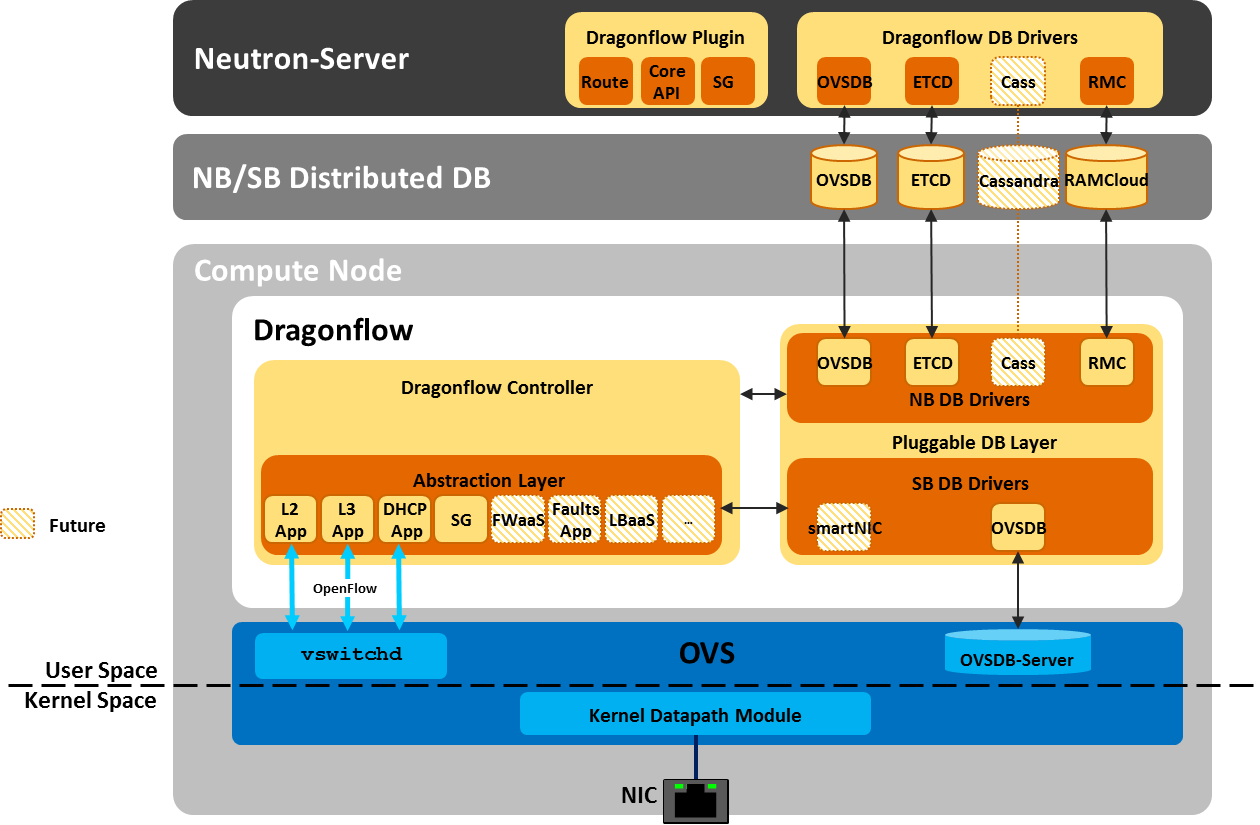
\includegraphics[width=\textwidth]{img/dragonflow_distributed_architecture.png}
\end{figure}

コンテナ、NAT、障害検知などもロードマップに入っています。RJ45がドラゴンの口に見える、というのはまぁ、気持ちは分かりますが。

\section{Freezer}

\begin{description}
	\item[wiki:] \url{https://wiki.openstack.org/wiki/Freezer}
	\item[IRC:] \verb|#openstack-freezer|
\end{description}

\begin{wrapfigure}[6]{r}[0mm]{0.3\textwidth}
	\begin{center}
		
\includegraphics[width=0.3\textwidth]{img/freezer_logo.png}
	\end{center}
\end{wrapfigure}

バックアップサービスです。複数のOSをサポートし(Linux・Windows・OSX・*BSD)、ブロックストレージのバックアップやファイルシステムの差分バックアップを可能にすることが目標です。また、指定時間での6ックアップやジョブの同期など、バックアップスケジューリングもスコープに含みます。暗号化もできるので安心です。さまざまなバックアップ技術が使用可能です。

\begin{itemize}
	\item セグメントサイズ(バックアップに使用するメモリ容量)
	\item キューサイズ(IOや帯域、メモリ・CPUの制限に応じて可変)
	\item バックアッププロセスの優先度
	\item 帯域制限
	\item 暗号化(AES-256-CFB)
	\item 圧縮(zlib・bzip2・xz/lzmaなど)
	\item 並列アップロードやさまざまなストレージメディアに対応(SwiftやSSHでリモートホストへの転送など)
	\item ファイルベースの差分バックアップ(\verb|tar|など)、ブロックベースの差分バックアップ(\verb|rsync|など)
	\item マルチプラットフォーム対応(LinuxではLVMなど、WindowsではVSSを用いる)
	\item 自動バックアップファイルローテーション
	\item バックアップ前後でのタスク実行
	\item 複数ノードでの同期バックアップ・リストア
\end{itemize}

Horizonとの統合も開発が進んでおり、CLIでできることがHorizonでもできるようになる予定です。以下のプロセスで構成されています。

\begin{description}
	\item[API:] REST APIの応答とスケジューラーへ受け渡しを担当します。実際のバックアップ作業は行わず、Schedulerに必要な情報を受け渡し、その結果を返すだけです。
	\item[Agent:] データをバックアップしたいリースで動くエージョンと型のプロセスです。実際にバップアップを実行します。単体で動かすこともできますが、Schedulerにより開始されることもあります。
	\item[Scheduler:] データをバックアップしたいノードで稼働する、Agentを管理するプロセスです。APIサーバーからの依頼を受け付け、バックアップ作業前後のタスクなどを担当します。Agentの動作状況を監視し、APIに返答します。並列バックアップのスケジューリングを担当します。
\end{description}

ノードで稼働するプロセスの存在が気にはなりますが、それもSSH経由などでリモートから可能であれば、十分実用可能性があると思います。オンプレ製品などにインストールするのは気が引けますね。

\section{Karbor}

\begin{description}
	\item[wiki:] \url{https://wiki.openstack.org/wiki/Karbor}
\end{description}

旧Smaugです。WikiにはOpenStackデプロイのデータとメタデータを保護するもの、あるいはKeystoneのプロジェクト下にあるものの保護、と書いてありますがこれだけではどうにもピンときません。

例えば以下のようなアプリケーションがあったとします。

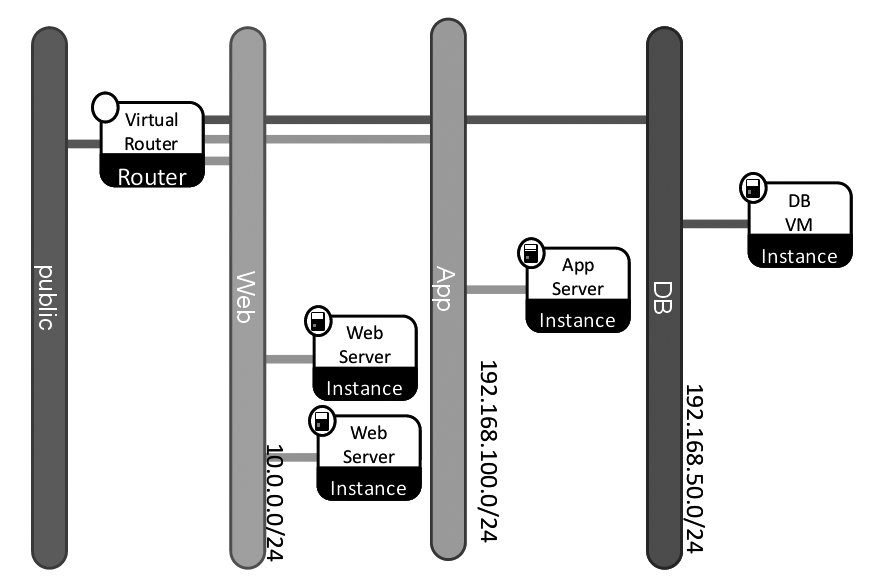
\includegraphics[width=\textwidth]{img/Smaug-sample-application.png}

このアプリケーションをシステムまるごと保存し、変更されたことを検知したいとします。このシステムを説明すると

\begin{itemize}
	\item DBインスタンスは1つで、DBネットワークに接続されている
	\item DBネットワークはRouter配下にある
	\item Appインスタンスは1つで、Appネットワークに接続されている
	\item AppネットワークはRouter配下にある
	\item Webインスタンスは2つあり
\end{itemize}

などなど、これらの情報を保存しておくことになります。Karborではこれを依存グラフとして表現します

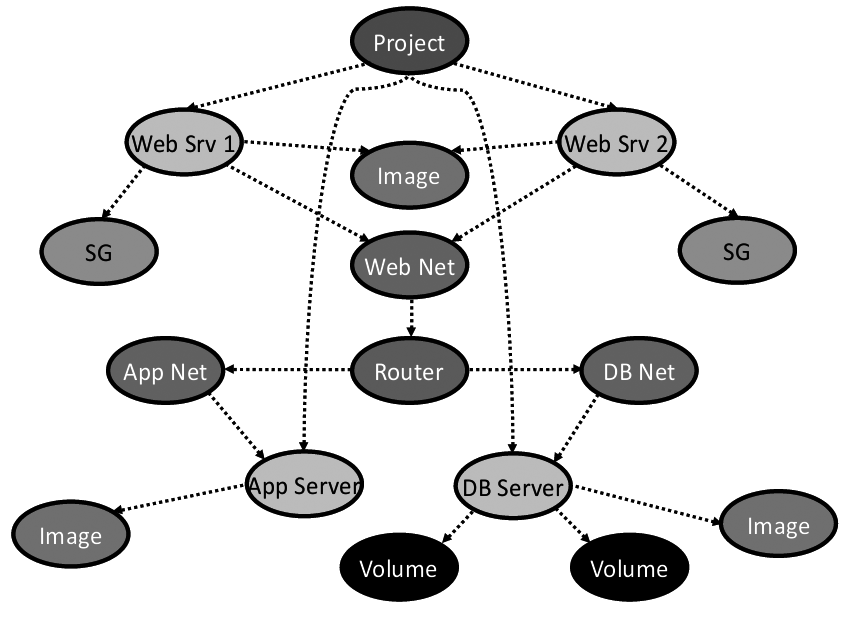
\includegraphics[width=\textwidth]{img/Smaug-dependency-graph.png}

Wikiを見ると分かりますが、割と複雑なシステム構成になっており、デプロイするだけでも大変そうです。コンポーネントが疎結合で、組み合わせることでシステムを作っていく指向とは逆行しそうですが、まぁクラウドエンタープライズ色がかなり強いプロジェクトですね。

\section{Kolla}

\begin{description}
	\item[wiki:] \url{https://wiki.openstack.org/wiki/Kolla}
	\item[wiki:] \url{http://docs.openstack.org/developer/kolla/}
	\item[IRC:] \verb|#openstack-kolla|
\end{description}

OpenStackのコンポーネントをDocker化しようというプロジェクトです。OpenStackのAPIサーバーはImmutableなものとして扱うことが容易なので、すでにコンテナを使っている人も多いのではないかと思います。MissionにはOpenStackデプロイの簡素化や素早い増強ができるようにするとあります。

特にカスタマイズしなくても動くようなイメージを目指しているようですが、DockerfileをJinja2のテンプレートになっているのでカスタマイズが可能です。ソースコードからのインストール、RDOやUbuntuのリポジトリを使ったインストールの両方をサポートしています。

コアコンポーネントだけでなく、CephやManila、Kuryrなどもデプロイできるようです。Kibanaもデプロイできるようで、これはOpenStackの監視に使う目的でしょう。

\section{Kuryr}

\begin{description}
	\item[wiki:] \url{https://wiki.openstack.org/wiki/Kuryr}
	\item[wiki:] \url{http://docs.openstack.org/developer/kuryr/}
	\item[IRC:] \verb|#openstack-kuryr|
\end{description}

\begin{wrapfigure}[13]{r}[0mm]{0.3\textwidth}
	\begin{center}
		
\includegraphics[width=0.3\textwidth]{img/kuryr_logo.png}
	\end{center}
\end{wrapfigure}

コンテナ用に設計されたNeurtonプラグインを作るプロジェクトです。Dockerのlibnetworkドライバ実装の1つという位置付けです。MagnumとNeutronの間の仲をとりもつ、という趣旨もあるようです。OpenStackを使ってコンテナのマネジメントをするために、必要ならNeutronあるいはDockerコミュニティーに対して働きかけたりするようです。Kuryr自体がコンテナネットワーク実装の唯一解になるつもりはないそうです。

コンテナに関しては長らくすったもんだを繰り返していましたが、ネットワークはKuryrになんとか落ち着いていきそうです。コンテナ自体はMagnumで落ち着きそうですし、OpenStackとコンテナはなんとか落としどころを見つけたのでしょうか。そもそも、仮想マシン(インスタンス)とコンテナではライフサイクルが違う、ということに無理があったりはします。

ところで、どう発音すればよいのかは謎である。くりあー?くりゅあー?

\section{Monasca}

\begin{description}
	\item[wiki:] \url{https://wiki.openstack.org/wiki/Monasca}
	\item[IRC:] \verb|#openstack-monasca|
\end{description}

インスタンスのモニタリングし、アラートを出してくれるようなサービスを作るプロジェクトです。高可用性とスケーラビリティーの良さをうたっており、OPNFVからの注目が熱いプロジェクトです。以下のような特徴を持っています。

\begin{itemize}
	\item ハイパフォーマンス・スケーラブル・高可用
	\item REST API実装によるシンプルな動作
	\item マルチテナント対応
	\item リアルタイム性
	\item 複数のアラームの合成
	\item Nagiosや\verb|statsd|との連携
	\item オープンコミュニティーでの開発
\end{itemize}

構成は意外と複雑です。

\begin{figure}
	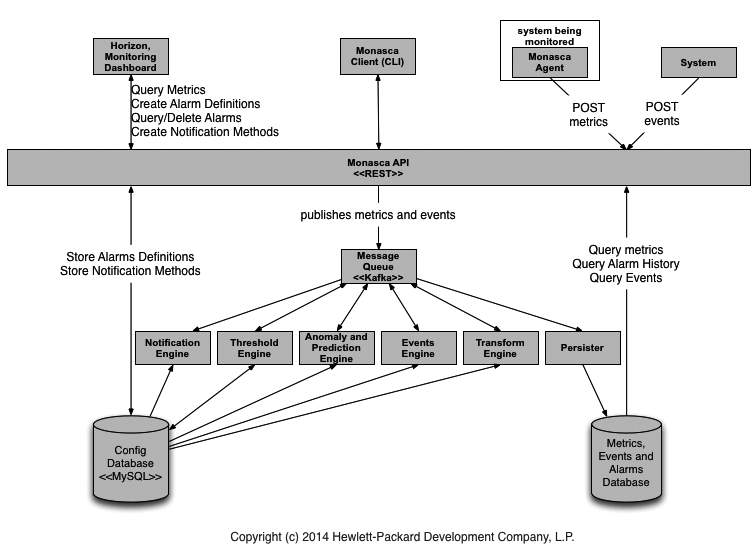
\includegraphics[width=\textwidth]{img/Monasca-arch-component-diagram.png}
\end{figure}

\begin{description}
	\item[Agent:] メトリクス監視エージェントです。MySQLなど有名所に対してはデフォルトである程度のアラートセットを定義済みです。Nagiosや\verb|statsd|との連携もできます。
	\item[Persister:] メッセージキューからのデータをデータベースに保管することに特化したプロセスです。大量のデータを高速に処理する必要があるので分離されているのでしょう。
	\item[UI:] Horizonに統合されています。モニタリングにはやはりGUIがあるべきでしょう。
	\item[Ceilometer Publisher:] Ceilometerとの連携機能もあります。
\end{description}

可用性とパフォーマンスにはかなり気を遣っているようです。既存のモニタリングシステムとの連携も考えられているようなので、段階的な導入はできそうな気がします。

\section{Searchlight}

\begin{description}
	\item[wiki:] \url{https://wiki.openstack.org/wiki/Searchlight}
	\item[wiki:] \url{http://docs.openstack.org/developer/searchlight/}
	\item[IRC:] \verb|#openstack-searchlight|
\end{description}

確か最初はGlanceのイメージを検索できるように、というような趣旨のプロジェクトだった気がするのですが、LibertyでのデザインサミットでGlanceに限らずOpenStackのリソースすべてを検索対象とする方針の転換がありました。今はサーチサービスという大義のようです。ミッションは「マルチテナンシーのある、スケーラブルなインデクサーとサーチエンジンの提供」です。

\begin{figure}
	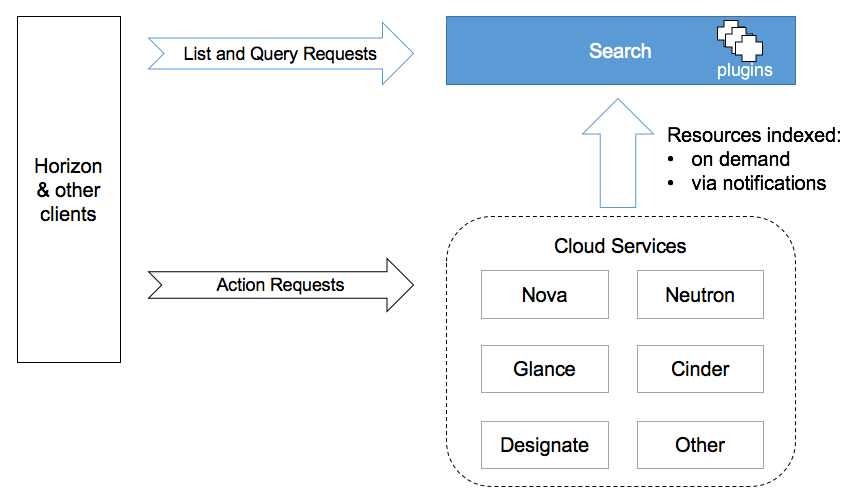
\includegraphics[width=\textwidth]{img/Searchlight-Concept-1.png}
\end{figure}

OpenStackにかかわるあらゆるもの、例えばインスタンスなどの情報を集めて、Elasticsearchにインデックスし、それを検索可能にするAPIを提供します。Horizonのインスタンス検索機能は貧弱ですし、APIも文字列部分一致程度のリスティング機能しかありませんので、Searchlightは便利だと言えるでしょう。

\section{Senlin}

\begin{description}
	\item[wiki:] \url{https://wiki.openstack.org/wiki/Senlin}
	\item[wiki:] \url{http://docs.openstack.org/developer/senlin/developer/index.html}
	\item[IRC:] \verb|#senlin|
\end{description}

インスタンスをクラスタ化することができるAPIを提供します。Novaが作成したインスタンスだけが対象ではなく、Heatのスタックなどもクラスタ化することができます。Heatで頑張ればなんとかできる、をSenlinでちゃんとやる、という感じです。

以下のような構成で動作します。

\begin{figure}
	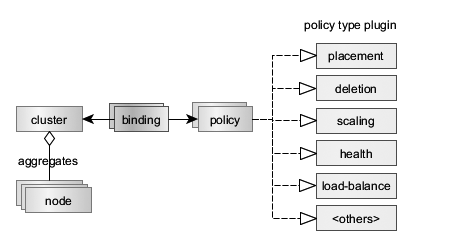
\includegraphics[width=\textwidth]{img/Senlin-policies.png}
\end{figure}

クラスタを管理するにおいて、ポリシーを設定することができ、以下のプラグインがあるようです

\begin{itemize}
	\item 配置 (Placement)
	\item 削除 (Deletion)
	\item スケール (Scaling)
	\item ヘルスチェック (Health)
	\item ロードバランシング
	\item その他
\end{itemize}

これらのポリシーに紐付けられたノードをまとめて管理することでクラスタを生成します。

\section{Solum}

\begin{description}
	\item[wiki:] \url{https://wiki.openstack.org/wiki/Solum}
	\item[wiki:] \url{http://docs.openstack.org/developer/solum/index.html}
	\item[IRC:] \verb|#solum|
\end{description}

Software Development Lifecycle Automation service: 直訳するとソフトウエア開発サイクルの自動化サービス、です。ソースコードのOSイメージへの配置やデプロイ作業を自動化し、OpenStackをアプリケーション開発フローと統合させることがミッションです。

プロジェクトのゴールは開発者目線からとアプリケーションの可搬性、アプリケーションを作成するプログラミング言語に依存しない設計の3つから定められています。

\subsection*{開発者の生産性}
\begin{itemize}
	\item 開発・テスト・ステージング・本番、などの環境を意識できるアプリケーションサイクルの管理ができる
	\item 自動化されたデプロイフローによるCI/CD環境の構築
	\item \verb|git push|
	\item IDE連携
\end{itemize}

\subsection*{アプリケーションの可搬性}
\begin{itemize}
	\item Solumnで動くアプリケーションは、どのベンダーのOpenStackでも動く
	\item パブリッククラウドでもプライベートクラウドでも動く
	\item Novaベースでデザインされているため、Dockerに対応
\end{itemize}

\subsection*{言語・拡張性}
\begin{itemize}
	\item ランタイムをプラグイン形式にすることで、Solumn自体はアプリケーションを作成したのプログラミング言語に依存しない。
	\item アドオン型式なので、独自の拡張が可能
	\item つまり、ベンダー独自の拡張も可能ではある
\end{itemize}

NovaのDokcerを使う、という辺りに少し不安はあるものの、ニーズは大きそうなプロジェクトです。

\section{Vitrage}

\begin{description}
	\item[wiki:] \url{https://wiki.openstack.org/wiki/Vitrage}
	\item[wiki:] \url{https://github.com/openstack/vitrage/tree/master/doc/source}
	\item[IRC:] \verb|#openstack-vitrage|
\end{description}

\begin{wrapfigure}[7]{r}[0mm]{0.3\textwidth}
	\begin{center}
		
\includegraphics[width=0.3\textwidth]{img/Vitrage_logo_finaly.png}
	\end{center}
\end{wrapfigure}

OpenStackのアラートやイベントを可視化したり分析することで、トラブルを未然に防いだり、トラブルシューティングに役立てようとするプロジェクトです。アーキテクチャは以下のようになっています。

\begin{figure}
	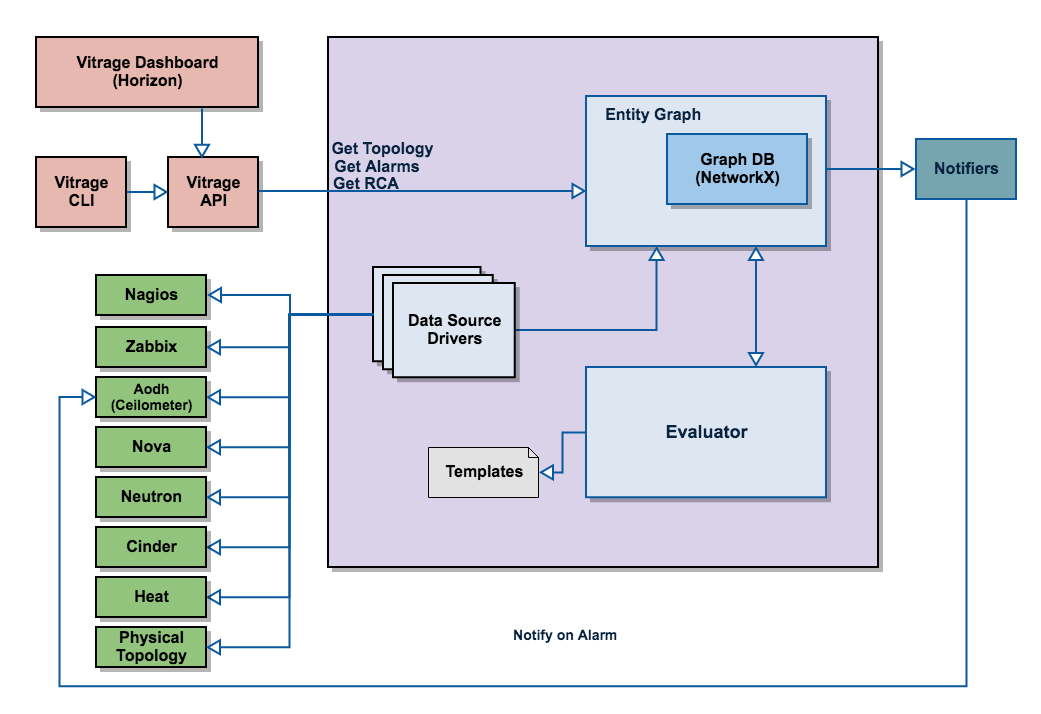
\includegraphics[width=\textwidth]{img/Vitrage-high_level_architecture2.png}
\end{figure}

以下のような機能を持っています。

\begin{itemize}
	\item コンピュートホストやネットワーク機器などの物理機器の状態と、その物理機に依存している仮想マシンとの紐付け
	\item 直接OpenStackを監視するのではなく、システムの分析をベースにした状態の変化やアラーティング
	\item アラートやイベントによる問題解決
	\item ダッシュボード (Horizon)
\end{itemize}

とあるネットワークスイッチで障害が発生した場合、どの仮想マシンが影響を受けるか、といった分析が可能になります。これらの情報を持っていることで、物理機器のメンテナンス時の影響を把握することも簡単になりそうです。

\section{Watcher}

\begin{description}
	\item[wiki:] \url{https://wiki.openstack.org/wiki/Watcher}
	\item[wiki:] \url{http://docs.openstack.org/developer/watcher/index.html}
	\item[IRC:] \verb|#openstack-watcher|
\end{description}

OpenStackベースのクラウド環境でのリソース制御機構を提供しようというプロジェクトです。システムメトリクスの収集や最適化、アクションプランのプロセスが動作します。データセンターの運用コストやマイグレーションによるシステムパフォーマンスの改善、電源効率の改善なども視野に入っているようです。制御アルゴリズムはデフォルトで入っているもの以外にもプラグイン形式で追加することもできます。OpenStack運用者のためのプロジェクトと言えます。なんともピンと来ませんが、いくつがユースケースが紹介されています。

\begin{itemize}
	\item サーバー筐体の温度や空調、電源管理などの物理的なリソースの運用時に、仮想マシンのホスト間移動や適切なスケジューリングの機構を提供する
	\item 最適化が必要になるしきい値の指定や変更が容易になる
	\item テストや開発環境ではリソースを詰めて、本番環境では少し余裕を持たせたスケジューリングをしたいなど、リソースセットを定義する
	\item リソースの使用状況を詳細に監視する
	\item イベントにはOpenStackのあらゆるコンポーネントに対応可能。 (Novaのマイグレーション、Keystoneの認証など)
	\item 逆にWatcherからイベントを発行させることも可能
\end{itemize}

以下のアーキテクチャで動作しています。例によって、メッセージキューによるイベント駆動になっています。また、データベースが2つあるようです。

\begin{figure}
	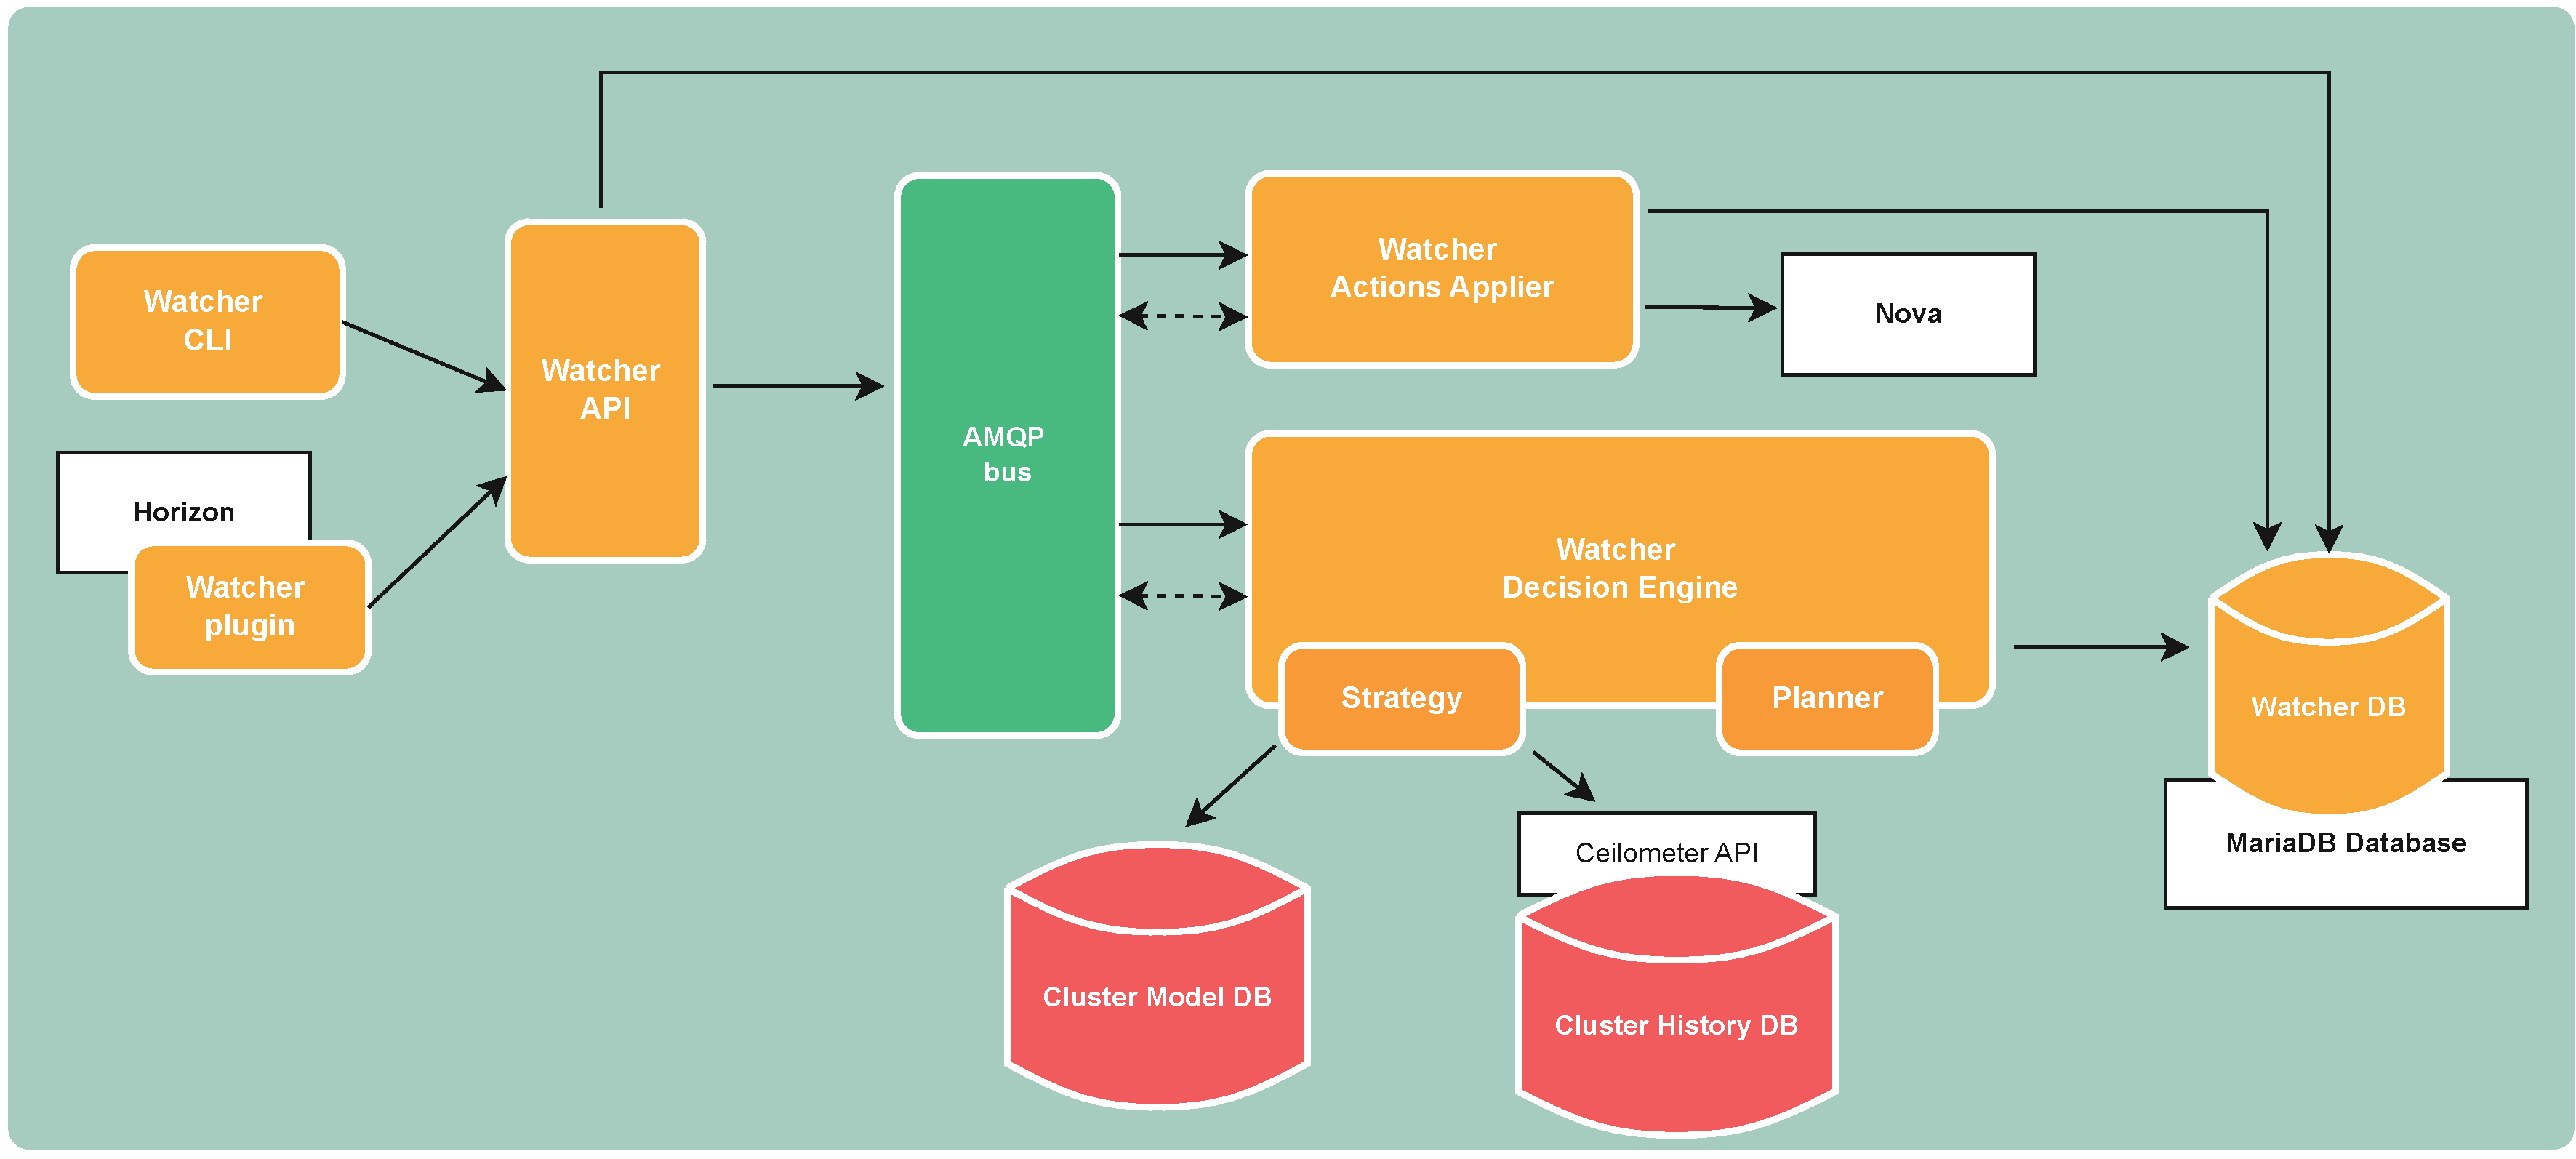
\includegraphics[width=\textwidth]{img/watcher-architecture.pdf}
\end{figure}

\begin{description}
	\item[API:] REST API実装です。実際のタスクは行いません。
	\item[Decision Engine:] Applierに渡すActionを作成します。「あるべき姿」にシステムを収束させるためのタスクを決定するプロセスになります。
	\item[Applier:] メッセージバスに接続され、Decision Engineが作成したプランを実際にプランを実行するプロセスです。タスクの失敗・成功を通知する機能があります。
	\item[Database:] Cluster History DBにはクラスタのメトリクスが保管されます。Ceilometerと似ています。Cluster Model DBにクラスタの情報は保管されるようです。
\end{description}
